%%% Pregunta 03:
Utilizando la tabla de traducci\'on entre una representaci\'on 
intermedia lineal y las instrucciones de arquitectura MIPS, 
genera el c\'odigo m\'aquina para la siguiente secuencia:

%! suppress = MissingLabel
\begin{lstlisting}
 d := c + 8
 a := a + b/$^{last}$/
 M[d/$^{last}$/] := a
 IF a < c THEN L1 ELSE L2
 LABEL L1
\end{lstlisting}

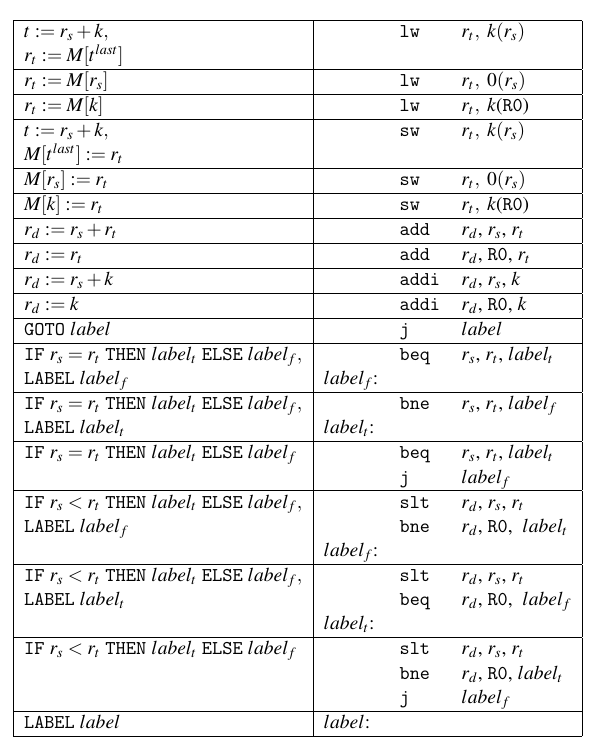
\includegraphics[width=.75\textwidth]{./MIPSInstrSet}

\begin{tabular}{l l}

    Secuencia Original & Código Maquina \\
     & \\
    $a \coloneqq a + b^{last}$ & $lw$ $\$1, a$
     & $lw$ $\$2, b^{last}$ \\
     & $add$ $\$3, \$1, \$2 $ \\
     & \\
    $d \coloneqq c + 8$ & \\
    $M[d^{last}] \coloneqq a$ & \\
     & $lw$ $\$4 , c$
     & $sw$ $\$3, 8(\$4)$\\
     & \\
    $IF$ $a < c$ $THEN$ $L1$ $ELSE$ $L2$ & \\
    $LABEL$ $L1$ & $L1: $ $slt$ $\$5, \$3, \$4$ \\
     & $beq$ $\$5, R0, L2$\\

\end{tabular}


\begin{lstlisting}


\end{lstlisting}
